

\begin{figure}[ht]

\begin{minipage}[c]{.38\linewidth}
\centering
    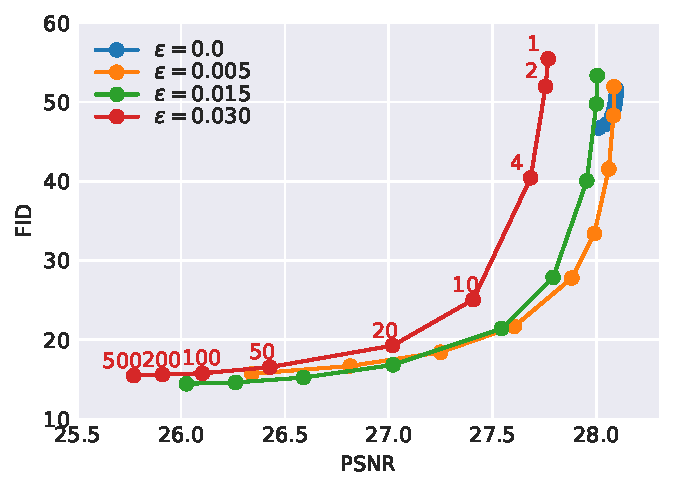
\includegraphics[width=\linewidth, clip=true, trim=5 0 0 0]{assets/pd_curve_sisrx4_fid_noise.pdf}\vspace{-.3em}

(a)
\end{minipage}
\begin{minipage}[c]{.61\linewidth}
\small
\centering
\setlength{\tabcolsep}{1pt}
\begin{tabular}{lcccccr}
\toprule
& Type & PSNR$\uparrow$ & LPIPS$\downarrow$ & FID$\downarrow$ & KID$\downarrow$ \\ \midrule
LDL(SwinIR)~\citep{liang2022details} & GAN	& 26.64	&	\colorbox{red!15}{0.102}	& \colorbox{red!15}{10.80} & \colorbox{red!15}{0.400} \\
LDL(RRDB)~\citep{liang2022details} & GAN &	26.43	&	\colorbox{blue!15}{0.109}	& \colorbox{blue!15}{11.36} & \colorbox{blue!15}{0.582}\\
ESRGAN~\citep{wang2018esrgan}	& GAN & 25.54	&	0.125	& 12.77 & 0.732	 \\
SRFLOW~\citep{lugmayr2020srflow}& NF	& 26.10	&	0.127	& 20.21 & 4.444 \\
BSRGAN~\citep{zhang2021designing}& GAN	& 24.35	&	0.241	& 31.43 & 5.229	\\
RRDB~\citep{wang2018esrgan}	& REG & \colorbox{red!15}{28.37}	&	0.264	& 50.98 & 19.000 \\
LIIF~\citep{chen2021learning}& REG	& \colorbox{blue!15}{28.15}	&	0.269	& 53.16 & 19.958 \\
BSRNET~\citep{zhang2021designing}& REG	& 25.90	&	0.348	& 84.11 & 36.901 \\
Ours (100 steps, $ \epsilon=0.015$)	&	& 26.45	& 0.136	& 15.39	& 1.761  \\
\bottomrule
\end{tabular}
\vspace{.2em}

(b)
\end{minipage} \vspace{-.5em}
\caption{$4\times$ Super-resolution on div2k dataset~\citep{div2k}. \colorbox{red!15}{Best values} and \colorbox{blue!15}{second-best values} for each metric are color-coded} 
\label{tab:sisr_4x}
\end{figure}


